\chapter{Inequações}

\section{Introdução}

As soluções de equações polinomiais têm um número finito de soluções. As de 1º Grau têm uma, as de 2º Grau podem ter até duas, e assim por diante. Outros problemas podem ter infinitas soluções:

Observe os seguintes exemplos:

\begin{texemplo}
Quantos alunos na sua turma têm mais de \textit{20 anos?}

Solução: evidentemente a solução depende da idade dos alunos da turma. Porém, podemos afirmar que podem ocorrer diferentes tipos de soluções:

\begin{enumerate}
	\item Nenhum aluno tem mais de 20 anos. Se \textit{x }é o número de alunos com mais de \textit{20} anos, a solução é \textit{S = $ \{ $ $ \} $ .}

	\item Existe um número finito de alunos com mais de 20 anos. Nesse caso, S = $ \{ $ x/ x > 0$ \} $ \qedsymbol{} 
\end{enumerate}
\end{texemplo}

\begin{texemplo}
Existe algum número real cujo dobro mais cinco seja maior do que zero? Quantos? Quais ?

Solução: Seja \textit{x o número procurado. Podemos escrever $``$dobro de x mais cinco seja maior do que zero$"$  em linguagem matemática:}

\textit{2x + 5 > 0. }

Não é difícil verificar que existem infinitos \textit{x reais que satisfazem esta desigualdade: -1, 0 , $\frac{1}{2}$, 1 , 2, 3, ....}

Observe (fazendo testes particulares) que se \textit{x = - 5/2, temos 2x + 5 = 0 e que }

se \textit{x < - 5/2~ temos 2x + 5 < 0 e que }

se \textit{x > - 5/2~ temos 2x + 5 > 0 .}

Assim, podemos concluir que \textit{S = $ \{ $ x  / x > -5/2$ \} $ \qedsymbol{}}
\end{texemplo}

Neste capítulo vamos aprender operar com desigualdades e resolver com segurança problemas semelhantes ao Ex.1.2.

\section{Inequações: definição e propriedades}

\begin{tdefinicao}
    Uma inequação é uma desigualdade de duas expressões matemáticas.
\end{tdefinicao}

\textbf{Exemplos:}

a) $-x +5 > x -\frac{1}{3}$

b) $x^{2} +2\leq 1$

c)  \( \frac{x}{2}+\frac{x-1}{3} \geq 3 \) \qedsymbol{}

A desigualdade numérica $2 < 3$ é verdadeira. Observe as seguintes operações:

\begin{enumerate}
	\item Adicionando 10 em ambos os lados da desigualdade, temos: 

\textit{2 + 10 <  3 + 10}

\textit{12~<~13.~   A nova desigualdade permanece verdadeira.}

	\item Adicionando -10 em ambos os lados da desigualdade, temos: 

\textit{2 + (-10)~~<  3 +(-10)}

\textit{-8~~<~-7.~   A nova desigualdade permanece verdadeira.~ }

	\item Multiplicando 10 em ambos os lados da desigualdade, temos: 

 \textit{2 $ \cdot $  10~~<  3~$ \cdot $   10}

\textit{20~<~30.~   A nova desigualdade permanece verdadeira.~ }

	\item Multiplicando -10 em ambos os lados da desigualdade, temos: 
\end{enumerate}

\textit{2 $ \cdot $  (-10)~~<  3 $ \cdot $  (-10)}

\textit{-20~<~-30.~   A nova desigualdade NÃO PERMANECE VERDADEIRA! }

Observe que, com exceção do produto por número negativo, opera-se com as inequações de forma semelhante às equações. Veja a seguir as propriedades das inequações.

\textbf{Propriedades das inequações:}

\begin{caixa}

Sejam \textit{u, v e w números reais ou variáveis e c um número real.}
\begin{enumerate}[label*=\arabic*.]
	\item \textbf{Transitiva:~}Se~ \textit{u~< v  }e \textit{v < w}~~ então \textit{u < w}. Ou
Se~ \textit{u >~v  e v > w~~ então u > w.}

	\item \textbf{Adição:} Se~ \textit{u~< v  }, então  \textit{u $ \pm $  w < v $ \pm $  w}~~ . Ou
Se~ \textit{u >~v  , então~ u $ \pm $  w > v $ \pm $  w~ .}

	\item \textbf{Multiplicação}:  Se~ \textit{u~< v  }e \textit{c > 0 }~~ então  \textit{u $ \cdot $  c  < v $ \cdot $  c}. 
Se~ \textit{u~< v  e \textbf{c < 0 ~~ então~ u~$ \cdot $  c  > v $ \cdot $  c.}}

\end{enumerate}

\end{caixa}

\begin{texemplo}
    Dada a desigualdade \textit{5 > 3, verifique se as desigualdades permanecem verdadeiras após a operação proposta:}

\begin{enumerate}
	\item Adicionar +4 em ambos os lados.

	\item Adicionar - 4  em ambos os lados.

	\item Multiplicar por (+2) em ambos os lados.

	\item Multiplicar por (-2) em ambos os lados.
\end{enumerate}

\textbf{Solução: }

\begin{enumerate}
	\item \textit{5+4 > 3+4}

\textit{9 > 7 . A desigualdade permanece verdadeira. (Propriedade da adição)}

	\item \textit{5 - 4 > 3 - 4}

\textit{1 > -1 . A desigualdade permanece verdadeira. (Propriedade da adição)}

	\item \textit{5~ $ \cdot $  (+2)  > 3 $ \cdot $  (+2)}

\textit{10 > 6 . A desigualdade permanece verdadeira. (Propriedade da Multiplicação por um número positivo)}

	\item \textit{5~ $ \cdot $  (-2)  > 3 $ \cdot $  (-2)}
\end{enumerate}

\textit{-10 > -6 . A desigualdade NÃO permanece verdadeira.}

Nesse caso, para que a igualdade fique verdadeira é necessário \textbf{INVERTER A DESIGUALDADE: (Propriedade da Multiplicação por um número NEGATIVO):}

\textit{-10 < -6 \qedsymbol{}}
\end{texemplo}

As propriedades das desigualdades são usadas para resolver inequações, como veremos nos próximos itens.

\begin{exercicios}
	\exitem{Dada a desigualdade 1 < 2 (que é verdadeira):}

\begin{enumerate}
	\item Adicionando -5 em ambos os lados, a desigualdade permanece verdadeira?

	\item Multiplicando ambos os lados por (+5), a desigualdade permanece verdadeira?

	\item Multiplicando ambos os lados por (-5), a desigualdade permanece verdadeira?
\end{enumerate}

    \exitem{Sejam M, N e P três números reais.}

\begin{enumerate}
	\item Se M > N~ e N > P , o que se pode afirmar sobre M e P ?

	\item Se M < N~ e N < P , o que se pode afirmar sobre M e P ?
\end{enumerate}

    \exitem{Compare as propriedades das equações com as das inequações. Em que operação elas se diferenciam?}

    \exitem{} Dada a inequação \textit{3x + 4 < 0}. A inequação é verdadeira para:

    a) \textit{x = 1} ?
    
    b) \textit{x = -2} ?
    
    c) \textit{x = -4/3}?
    
    d) \textit{x = -3} ?

	\exitem{} Dada a inequação $-x + 2 \geq 0 $. A inequação é verdadeira para:

    a) \textit{x = 1} ?
    
    b) \textit{x = 2} ?
    
    c) \textit{x = 3} ?
    
    d) \textit{x = -3} ?

	\exitem{} Use as propriedades da adição e multiplicação para que o lado direito das inequações torne-se nulo: 

	a) \textit{x + 2 > -x +3}

	b) \textit{2 + 3x < 4x +1}
    
    c) \( \frac{1}{2}+2x \geq \frac{4}{3} \)

    d) \( \frac{3}{4}x-\frac{2}{3} \leq 2 \)

	\exitem{} Use as propriedades da adição e multiplicação para isolar \textit{x} do lado esquerdo da inequação: 

    a) \textit{3x - 8 < x + 4}

    b) \textit{2x - 12 < 4x + 6}
    
    c) \( 3+\frac{1}{2}x \geq 5x \)
    
    d) \( \frac{x+1}{4} \leq \frac{x-1}{2} \)

\item Verifique se as afirmações abaixo são verdadeiras. Justifique sua resposta. Considere \textit{a um número real.}

a) $a^{2} > 0 => a > 0$

b) $a > 3  => a \geq 3$

c) $a3 > 0 => a > 0$

d) $a \geq ~3 => a > 3$

\end{exercicios}

\section{Inequações de 1º Grau}

\begin{caixa}

\begin {tdefinicao}
Uma inequação do primeiro grau é uma desigualdade de expressões algébricas que pode ser reduzida à forma
\textit{ax + b < 0~ , para a $ \neq $  0. }

\textbf{OBSERVAÇÃO: Onde foi usado\textit{ $``$<$"$  pode ser também $``$>$"$ , $``$$ \leq $ $"$ ~ ou~~$``$$ \geq $ $"$  .  }}
\end{tdefinicao}
\end{caixa}

\begin{texemplo}
Resolva a inequação~ \textit{- x +5 < 3x -~4  para x  R.}

\textbf{Solução:} Resolver uma inequação significa determinar os possíveis valores da incógnita (nesse caso \textit{x) que satisfazem a desigualdade. Faremos isso de forma semelhante às equações, porém usando as propriedades das inequações.}

Para termos \textit{x apenas do lado esquerdo, podemos adicionar (-3x) em ambos os lados da desigualdade (Propriedade da Adição):}

\textit{(-3x)- x +5 < (-3x)+3x - 4}

\textit{-4x +5 <~ - 4.}

Para termos apenas números no lado esquerdo, podemos adicionar (\textit{-5) em ambos os lados da desigualdade (Propriedade da Adição):}

\textit{-4x +5 + (-5) <~ - 4+(-5).}

\textit{-4x  <~ - 9.}

Finalmente, para termos apenas \textit{x no lado esquerdo, multiplicamos a inequação por (-1/4) e invertemos a desigualdade, pois -1/4 < 0. (Propriedade da multiplicação)}

 \[  \]  \[ -4x \cdot  \left( -\frac{1}{4} \right) > -9 \cdot  \left( -\frac{1}{4} \right)  \] 

\textit{x > 9/4 . Portanto, S=$ \{ $ x 	$\in$  \textbf{R / x > 9/4 $ \} $ .}}

Representando a solução na reta real, temos:\textit{}

\begin{figure}[H]
	\centering
		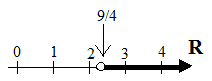
\includegraphics[width=1.77in,height=0.54in]{capitulos/inequacoes/media/image2.png}\qedsymbol{}
\end{figure}
\end{texemplo}

\begin{texemplo}
Resolva a inequação   \( \frac{x}{2} \geq \frac{3x+1}{3} \) \textit{ para x  R.}

\textbf{Solução:} Para evitar trabalhar com denominadores, multiplicamos a inequação por (\textit{6). (Propriedade da multiplicação)}

 \[  \]  \[ 6 \cdot \frac{x}{2} \geq \frac{3x+1}{3} \cdot 6 \] 

\textit{3x~ $ \geq $ ~ 6x + 2 . Adicionamos (-6x) (Propriedade da Adição)}

\textit{-3x~ $ \geq $ ~ 2 . Dividimos por (-3) (Propriedade da Multiplicação por número negativ2o)}

 \( x  \leq  -\frac{2}{3} \) ~~.  Portanto, \textit{S=$ \{ $ x $\in$ \textbf{R / x $ \leq $  -2/3 $ \} $ . }}

Representando a solução na reta real, temos:

\begin{figure}[H]
	\centering
	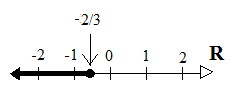
\includegraphics[width=1.79in,height=0.79in]{capitulos/inequacoes/media/image3.png}\qedsymbol{}
\end{figure}

\end{texemplo}

\textbf{Solução da inequação de primeiro grau com o lado direito nulo }

A resolução de uma inequação do 1º Grau também pode ser obtida utilizando a redução à forma \textit{ax + b < 0 , para a $ \neq $  0. O sinal da desigualdade pode ser também $``$>$"$ , $``$$ \leq $ $"$ ~ ou ~$``$$ \geq $ $"$  .  Observemos que sempre é possível escrever essa forma com a > 0. Por exemplo, }

Se temos  \textit{~ -2x + 5 > 0~~ podemos multiplicar por (-1) obtendo, 2x - 5 < 0.~~ }

\begin{caixa}

Os seguintes passos levam à solução da inequação de 1º Grau: 

1º ) Passo: Encontrar a solução da equação correspondente \textit{ax + b = 0 que é~~ x = -b/a.}

2º ) Passo: Verificar o sinal da desigualdade :

\begin{enumerate}
	\item Se for $``$>$"$  então a solução da inequação é:  \textit{S=}$ \{ $ \textit{x $\in$ } \textbf{\textit{R}} \textit{/ x >~ -b/a} $ \} $ 

	\item Se for $``$<$"$  então a solução da inequação é:  \textit{S=}$ \{ $ \textit{x $\in$ } \textbf{\textit{R}} \textit{/ x <~ -b/a} $ \} $ 

	\item Se for \textit{$``$$ \leq $ $"$ } então a solução da inequação é:  \textit{S=}$ \{ $ \textit{x $\in$ } \textbf{\textit{R}} \textit{/ x $ \leq $ ~ -b/a} $ \} $ 

	\item Se for \textit{$``$$ \geq $ $"$ } então a solução da inequação é:  \textit{S=}$ \{ $ \textit{x $\in$ } \textbf{\textit{R}} \textit{/ x $ \geq $ ~ -b/a} $ \} $ 
\end{enumerate}
\end{caixa}

\begin{texemplo}
    Resolva a inequação \( \frac{x}{2} \geq \frac{3x+1}{3} \) \textit{ para x  R reduzindo a inequação à forma ax + b $ \leq $   0.}

\textbf{Solução:} Multiplicando a inequação por (\textit{6) e adicionado (-6x), obtemos (ver Ex. 3.2):}

\textit{3x~ $ \geq $ ~ 6x + 2 . Adicionando (-6x -2),~obtemos  }

\textit{-3x -2  $ \geq $ ~ 0. Multiplicnado por (-1), obtemos~~~  }

\textit{3x +2~ $ \leq $ ~ 0. A~inequação~está na forma   ax + b $ \leq $   0~~ com a > 0 .}

1º) Passo: A solução da equação correspondente é \textit{x = -2/3.}

2º) Passo: o sinal da inequação com \textit{a > 0~~ é $``$$ \leq $ $"$ . Então a solução é (iii):}

\textit{S=$ \{ $ x $\in$  \textbf{R / x~$ \leq $   -2/3 $ \} $  \qedsymbol{}}}
\end{texemplo}

\begin{texemplo}
Resolva a dupla inequação \( -\frac{3}{2} \leq \frac{x+1}{2}<2 \) \textit{ para x  R.}

\textbf{Solução:} Usaremos as propriedades das inequações para isolar \textit{x entre as desigualdades. Para evitar os denominadores, multiplicamos a dupla inequação por 2.}

\textit{- 3  $ \leq $  ~ x+1  <  4.  Adicionando (-1) em cada membro, temos:}

\textit{- 3 +(-1) $ \leq $  ~ x+1 +(-1) <  4+(-1)}

\textit{- 4  $ \leq $  ~ x  <  3. Portanto, S=$ \{ $ x $\in$ \textbf{R / -4  $ \leq $  ~ x  <  3$ \} $ . }}

Representando a solução na reta real, temos:

\begin{figure}[H]
		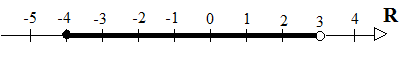
\includegraphics[width=4.2in,height=0.64in]{capitulos/inequacoes/media/image4.png}\qedsymbol{}
	\centering
\end{figure}
\end{texemplo}

\begin{exercicios}
	\exitem{Resolva as inequações do primeiro grau usando as propriedades:}

	a) \textit{2x - 1 $ \leq $  3x +3 }

    b) \textit{2(5 - x) + 2(3x-1) $ \geq $  2x + 1 }
    
    c)  \( \frac{5x+7}{4} \leq -2 \)
    
    d) \( \frac{2-x}{3}+\frac{3x-1}{2}<-1 \)

	\item Represente as soluções do Exercício anterior na reta real.

	\exitem{Resolva as inequações de primeiro grau anulando o lado direito:}

	a) \( \frac{x-2}{3}+\frac{x+2}{3}<2 \)

    b) \( \frac{2x-1}{5} \leq \frac{x+3}{2}+3x \)
    
    c)  \( \frac{1}{6}+\frac{x+1}{3}>\frac{2}{3} \)
    
    d)  \( \frac{3x+1}{3} \geq \frac{x-3}{4}-\frac{3x+1}{6} \) 

    \exitem{Resolva as inequações duplas de primeiro grau:}

	a) 2 \textit{$ \leq $ ~ x~+ 6  < 9}

    b)  \( 4 \geq \frac{y-3}{5} \geq -1 \)
    
    c) -1 \textit{$ \leq $ ~ -3x~+ 2  < 5}
    
    d)  \( -2 \leq \frac{2t+3}{3} \leq \frac{5}{4} \)

	\item Represente as soluções do Exercício anterior na reta real.
\end{exercicios}

\section{Inequações do 2º Grau}

\begin{caixa}
\begin{tdefinicao}
 Uma inequação do segundo grau é uma desigualdade de expressões algébricas que pode ser reduzida à forma

$ax^{2} + bx + c < 0$ para a $ \neq $ 0.

\textbf{OBSERVAÇÃO: Onde foi usado \textit{$``$<$"$  pode ser também $``$>$"$ , $``$$ \leq $ $"$ ~ ou~~$``$$ \geq $ $"$  .  }}

\end{tdefinicao}
\end{caixa}
A resolução de uma inequação do 2º Grau pode ser obtida utilizando a redução à forma 

$x^{2} + bx + c < 0$. (Onde foi usado $``$<$"$  pode ser também $``$>$"$ , $``$$ \leq $ $"$ ~ ou~ $``$$ \geq $ $"$ )

seguindo os seguintes passos:

\begin{caixa}

1º ) Passo: Encontrar as soluções reais (se existirem) da equação $ax^{2} + bx + c = 0$, que chamaremos $x_{1} e  x_{2}$ e consideraremos x1 < x2.

2º ) Passo: classificar as raízes:

\textbf{1º) Caso: raízes não reais (nesse caso o discriminante \textit{$b^{2}$ - 4ac < 0) }}

\begin{enumerate}
	\item Se o sinal da desigualdade for $``$<$"$  ou $``$\textit{$ \leq $ }$"$ , então \textit{S=}$ \{ $ $ \} $ 

	\item Se o sinal da desigualdade for $``$>$"$  ou $``$$ \geq $ $"$ , então \textit{S=}$ \{ $ \textit{x $\in$ } \textbf{\textit{R}}$ \} $ \textit{.}
\end{enumerate}

\textbf{2º) Caso: raízes reais idênticas: \textit{$x_{1} = x_{2}$ (nesse caso o discriminante $b^{2} - 4ac  = 0$) }}

\begin{enumerate}
	\item Se o sinal da desigualdade for $``$<$"$ , então \textit{S=}$ \{ $ $ \} $ 

	\item Se o sinal da desigualdade for $``$\textit{$ \leq $ }$"$ , então \textit{S=}$ \{ $ \textit{x $\in$ } \textbf{\textit{R }}\textit{/ x\textbf{ = }$x_{1}$} $ \} $ \textit{.}

	\item \textit{ }Se o sinal da desigualdade for $``$\textit{>}$"$ , então \textit{S=}$ \{ $ \textit{x $\in$ } \textbf{\textit{R }}\textit{/ x\textbf{ $ \neq $  }$x_{1}$} $ \} $ 

	\item  Se o sinal da desigualdade for $``$\textit{$ \geq $ }$"$ , então \textit{S=}$ \{ $ \textit{x $\in$ } \textbf{\textit{R}}$ \} $ 
\end{enumerate}

\textbf{3º) Caso: raízes reais distintas: \textit{$x_{1} \neq ~ x_{2}$ (nesse caso o discriminante $b^{2} - 4ac > 0$) }}

\begin{enumerate}
	\item Se o sinal da desigualdade for $``$<$"$ , então \textit{S=}$ \{ $ \textit{x $\in$ } \textbf{\textit{R }}\textit{/ $x_{1}$ < x < $x_{2}$}$ \} $ 

	\item Se o sinal da desigualdade for $``$\textit{$ \leq $ }$"$ , então \textit{S=}$ \{ $ \textit{x $\in$} \textbf{\textit{R }}\textit{/ $x_{1}$ $ \leq $  x $ \leq $  \textbf{ }$x_{2}$}$ \} $ 

	\item Se o sinal da desigualdade for $``$>$"$ , então \textit{S=}$ \{ $ \textit{x $\in$ } \textbf{\textit{R }}\textit{/ x < $x_{1}$} ou \textit{x >\textbf{ }$x_{2}$} $ \} $ 

	\item  Se o sinal da desigualdade for $``$\textit{$ \geq $ }$"$ , então \textit{S=}$ \{ $ \textit{x $\in$ } \textbf{\textit{R }}\textit{/ x $ \leq $ $x_{1}$} ou\textit{ x $ \geq $ $x_{2}$}$ \} $ 
\end{enumerate}

\end{caixa}

\begin{texemplo}
Resolva a inequação $x^{2} +2 x \leq 2x2+3 para x \in R$.

\textbf{Solução:} Precisamos reduzir a inequação dada à forma $ax^{2} + bx + c \leq$ ou $\geq 0$. Para isso, adicionamos (-2x2 - 3) em ambos os lados e obtemos:

\textbf{$-x^{2} + 2x - 3 \leq 0~$. Multiplicando por (-1), para que a > 0, temos:}

$x^{2} - 2x + 3 \geq 0$. \textbf{(Observe que o sinal da desigualdade ficou $``$$ \geq $ $"$ )}

1º) Passo: A equação  $x^{2} - 2x + 3 = 0$ não tem raízes reais.

2º) Passo: como as raízes não são reais, temos o 1º Caso. Como o sinal da desigualdade é  $``$\textit{$ \geq $ $"$ , temos a situação (ii). Então, a solução será:}

\textit{S=$ \{ $ $\in$ x  \textbf{R$ \} $ . Ou seja, qualquer número real satisfas a inequação dada \qedsymbol{}}}
\end{texemplo}

\begin{texemplo}
    Resolva a inequação $x^{2} - x < x+3$ para $x \in R$.

\textbf{Solução:} Precisamos reduzir a inequação dada à forma $ax^{2} + bx + c <$ ou $> 0$. Para isso, adicionamos ($-x-3$) em ambos os lados e obtemos:

\textit{$x^{2} - 2x - 3 < 0$}.

1º) Passo: As raízes da equação  $x^{2} - 2x - 3 = 0$ são $x_{1} = -1$ e  $x_{2} = 3.$

2º) Passo: como as raízes são reais e distintas, temos o 3º Caso. Como o sinal da desigualdade é~ $``$\textit{<$"$ , temos a situação (i). Então, a solução está entre as raízes:}

S=$ \{ x \in R / -1 < x < 3 \} $ \qedsymbol{}
\end{texemplo}

\begin{exercicios}
	\exitem{} Resolva as inequações de segundo grau para $x \in R $:

	a) \textit{x\textsuperscript{2} - 4x < 0}

	b) \textit{x\textsuperscript{2} - 4x + 3 > 0}

	c) \textit{x\textsuperscript{2} +6x + 9 < 0}

    d)\textit{x\textsuperscript{2} +4x + 4 $ \leq $  0}

    e) \textit{ x\textsuperscript{2} +2x + 1 $ \geq $  0}

    f)\textit{  x\textsuperscript{2} -~ 9 < 0}

    g) \textit{x\textsuperscript{2} -~ 9 > 0}

    h) \textit{x\textsuperscript{2} +~ 9 $ \leq $ 0}

    i) \textit{x\textsuperscript{2} -~ 9 $ \geq $  0}
	\item Represente as soluções do Exercício anterior na reta real.
\end{exercicios}

\section{RESPOSTAS DOS EXERCÍCIOS PROPOSTOS}

\begin{respostas}{2}
    \ansitem{a) Sim; b) Sim; c) Não}

    \ansitem{a) M > P; b) M < P}

    \ansitem{Na multiplicação de um número negativo por uma inequação deve-se inverter o sentido da desigualdade.}

    \ansitem{a) Não; b) Sim; c) Não; d) Sim}

    \ansitem{a) Sim; b) Sim; c) Não; d) Sim}

    \ansitem{}
    a) 2x -1 > 0
    
    b) -x +1 < 0
    
    c) 2x - 5/6 $ \geq $  0
    
    d) 9x -32 $ \leq $ 0

    \ansitem{}
    a) $x < 6$
    
    b) $x > -9$
    
    c) $x \leq \frac{2}{3}$
    
    d) $x \geq 3$
\end{respostas}

\begin{respostas}{3}
    \ansitem{}
    a) S=$ \{ x \in R / x \geq -4 \} $

    b) S=$ \{ x \in R / x \geq -7/2 \} $

    c) S=$ \{ x \in R / x \leq  3 \} $
    
    d) S=$ \{ x \in R / x < -1\} $

    \stepcounter{enumi}

    \ansitem{}
    a) $2x - 6 < 0$ e S=$\{x \in R / x < 3 \}$

    b) $31x + 17 \geq 0$ e S=$ \{x \in R / x \geq -17/31 \} $

    c) $2x - 1 > 0$ e S=$ \{ x \in R / x > 1/2 \} $

    d) $x + 1 \geq 0$ e S=$ \{ x \in R / x \geq -1 \} $

    \ansitem{}
    a) S=$ \{ x \in R / -4 \leq x < 3  \} $

    b) S=$ \{ y \in R / 17 \geq y \geq -2 \} $

    c) S=$ \{ x \in R / 1 \geq x > -1  \} $

    d) S=$ \{ t \in R / -9/2 \leq t \leq 3/8 \} $
\end{respostas}

\begin{respostas}{4}
    \ansitem{}
    a) S=$ \{ x \in R / 0 < x < 4 \}$

    b) S=$ \{ x \in  R / x < 1$ ou $x > 3 \}$

    c) S= $\emptyset$

    d) S=$ \{ -2 \} $

    e) S=$ \{ x \in R \} $ 

    f) S=$ \{ x \in R / -3 < x < 3 \}$

    g) S=$ \{ x \in R / x< -3$ ou $x> 3 \} $

    h) S=$ \{ x \in R / x \leq -3$ ou x $\geq 3 \} $

    i) S=$ \{ x \in R / x \leq -3$ ou x $\geq 3 \} $
\end{respostas}